\documentclass[
  listof=totoc,
  bibliography=totoc,
  12pt,
  % parskip=full,
  ]{scrreport}
\setuptoc{toc}{totoc}
% \usepackage[a4paper, total={6.5in, 10in}]{geometry}
\renewcommand{\baselinestretch}{1.5}

\usepackage{amsmath}
\usepackage[T1]{fontenc}
\usepackage[utf8]{inputenc}
\usepackage[spanish]{babel}
\usepackage{hyperref}
\hypersetup{
  pdftitle={Uso de bibliotecas de análisis y visualización
in-situ en una simulación sísmica numérica},
  pdfauthor={Christian Asch},
  colorlinks=true,
  breaklinks=true,
}
\usepackage[nameinlink, noabbrev, spanish]{cleveref}
\usepackage{csquotes}
\usepackage[backend=biber]{biblatex}
\usepackage{graphicx}
\usepackage{xcolor}
\usepackage{tikz}
\graphicspath{{./images/}}
\addbibresource{refs.bib}

\newbox\namebox
\newdimen\signboxdim

\def\signature#1{%
    \setbox\namebox=\hbox{#1}
    \signboxdim=\dimexpr(\wd\namebox+1cm)
    \parbox[t]{\signboxdim}{%
        \centering
%           \mbox{}\leaders\hbox to .4em{\hss.\hss}\hskip\nameboxdim\mbox{}\\   % for dots
            \hrulefill\\    % for a line
            #1
        \par}%
    }

\begin{document}

\begin{titlepage}
  \begin{center}
    UNIVERSIDAD DE COSTA RICA

    SISTEMA DE ESTUDIOS DE POSGRADO

    \vspace{2.5cm}
    Integración de bibliotecas de análisis y visualización in-situ en una simulación sísmica numérica.

    \vspace{2.5cm}
    Propuesta de tesis de maestría sometida a la consideración de la Comisión del Programa de Estudios de Posgrado en Computación e Informática para optar al grado y título de Maestría Académica en ciencias de la computación en informática.

    \vspace{2.5cm}
    CHRISTIAN ASCH BURGOS

    \vspace{4.5cm}
    Ciudad Universitaria Rodrigo Facio, Costa Rica

    2024

  \end{center}
\end{titlepage}

``Esta Propuesta de Tesis de Maestría será presentada a la Comisión de Estudios de Posgrado en Computación e Informática de la Universidad de Costa Rica, como requisito parcial para optar por el grado y título de Maestría Académica en Computación e Informática''


\begin{center}

    \signature{Nombre del representante}\\
    \vspace{0.5cm}
    Representante del decano\\
    Sistema de estudios de posgrado
    \vspace{0.70cm}


    \signature{Dr. Esteban Meneses}\\
    \vspace{0.5cm}
    Director de tesis
    \vspace{0.70cm}
    
    \signature{Dr. Silvio Rizzi}\\
    \vspace{0.5cm}
    Asesor
    \vspace{0.70cm}

    \signature{Dr. Edgar Casasola}\\
    \vspace{0.5cm}
    Asesor
    \vspace{0.70cm}

    \signature{Nombre del representante}\\
    \vspace{0.5cm}
    Representante del director\\
    Programa del Posgrado en Computación e Informática
    \vspace{0.70cm}

    \signature{Christian Asch}\\
    \vspace{0.5cm}
    Candidato

    
\end{center}

\pagenumbering{Roman}
\listoftables
\listoffigures
\tableofcontents

\chapter{Introducción}
\pagenumbering{arabic}
Los sismos son fenómenos con los que interactuamos con bastante frecuencia. Cada día, suceden aproximadamente 50 temblores perceptibles en el mundo~\cite{Shearer2019}. La ciencia que utilizamos para estudiar estos fenómenos es la sismología, esta es una ciencia moderna, que tiene sus inicios en las últimas décadas del siglo XIX, cuando Robert Mallet viajó a Nápoles para documentar la destrucción del terremoto de 1857. El trabajo de Mallet fue el primer paso para el estudio de los sismos de forma científica~\cite{Shearer2019}. Las ondas mecánicas generadas por los sismos nos ayudan a conocer la composición de las capas internas de la tierra, las cuales no podemos observar directamente. Esto se utiliza, por ejemplo, en la prospección de yacimientos petrolíferos. También, al conocer el comportamiento de las ondas generadas por temblores podemos detectar ondas artificiales, lo que da paso a la detección de pruebas nucleares~\cite{Shearer2019}.

En la ciencia, el uso de simulaciones permite comparar modelos con datos observados, esto sirve para evaluar los ámbitos en los que el modelo puede ser o no válido. En la sismología, existen métodos de simulación clásicos como lo es la teoría de rayos y las soluciones modales, que siguen siendo útiles e importantes debido a que son menos costosas computacionalmente. Gracias al avance en hardware y software, se ha hecho posible la aplicación de métodos numéricos que permiten el cálculo de sismogramas sintéticos y la resolución de problemas tridimensionales~\cite{Igel2016}. Las simulaciones en sismología son de gran importancia, ya que complementan los datos históricos y esto ayuda a la investigación, y a la toma de decisiones en áreas como lo es el diseño y la infraestructura. Un ejemplo de simulación es AWP-ODC, esta simulación hace uso del método numérico de diferencias finitas para resolver las ecuaciones diferenciales del modelo. Este software fue utilizado en el 2010 para simular sismos de magnitud 8 con una frecuencia de 2 Hz en el sur de California, abarcando un área de 800 km por 400 km en computadoras de petaescala~\cite{Cui2010}, capaces de realizar $10^{15}$ operaciones de punto flotante de 64 bits por segundo (FLOPS).

El TOP500 es el listado de las supercomputadoras más poderosas en el mundo, este se actualiza de manera semestral desde 1993. En el listado publicado en el primer semestre del 2008~\cite{top500}, la supercomputadora RoadRunner se convirtió en la primer computadora de petaescala, desde entonces se notaba que las unidades de entrada/salida (E/S) no estaban avanzando tan rápido como las unidades de procesamiento, por lo que podrían convertirse en cuellos de botella~\cite{Narayan2009}. Ya desde el 2007 el departamento de energía de los Estados Unidos (DoE) se empezó a preparar para el desarrollo de las supercomputadoras de exaescala, montando talleres para identificar los beneficios y retos que iban a traer, como lo es la E/S y los requerimientos energéticos del mantenimiento y uso de estos sistemas~\cite{Messina2017}. Se han propuesto múltiples soluciones al problema de la E/S, como lo es la E/S paralela~\cite{Byna2022} o el análisis y visualización in-situ~\cite{akira_kageyama_approach_2014}.

Tradicionalmente, el posprocesamiento de los datos de simulación se realiza una vez que esta ha finalizado de ejecutarse, lo que llamamos un procesamiento post-hoc~\cite{childs_terminology_2020}. En contraste, el análisis y visualización in-situ se refiere a realizar el procesamiento de los datos conforme son generados. Si los datos son procesados de forma local a la simulación, se puede evitar el escribirlos al disco por lo que es posible ahorrar tiempo en la E/S del sistema. Un ejemplo de esto es una versión de AWP-ODC que fue desarrollada con capacidades de análisis in-situ por medio de la biblioteca Catalyst. Esta versión del programa demostró un rendimiento aceptable en comparación a la versión original, con la ventaja adicional de haber reducido significativamente el tamaño de almacenamiento de la salida del programa~\cite{mu_-situ_2019}. Este estudio resalta los resultados prometedores y beneficiosos de utilizar bibliotecas en simulaciones numéricas de sismología para la investigación.

Otro aspecto beneficioso del análisis y visualización in-situ es la capacidad de dirigir computacionalmente las simulaciones~\cite{Grosset2020}. Tradicionalmente, las visualizaciones y métricas de simulación solo estaban disponibles después de que esta haya finalizado o alcanzado un punto de control. Sin embargo, el análisis y visualización in-situ permite que los resultados estén disponibles constantemente durante la simulación, lo que brinda a los investigadores la oportunidad de tomar decisiones anticipadas, como detener la simulación si comienza a divergir o si cambian las condiciones. Este tipo de interacción con las simulaciones se ha utilizado en otros dominios~\cite{Yi2014} y sería valioso para las simulaciones sísmicas.

\section{Aportes de la investigación}
Esta investigación tendrá tres aportes principales
\begin{itemize}
  \item Una caracterización de simulaciones en otras áreas de la ciencia que hagan uso de bibliotecas de análisis in-situ. Esto será valioso para futuros investigadores que vayan a implementar sistemas similares. 
  \item La creación de una simulación sísmica que haga uso del análisis y visualización in-situ, lo que permitirá que los investigadores del área puedan tener mayor control sobre la simulación, así como hacer un mejor uso de la infraestructura computacional de exaescala. 
  \item Una evaluación del rendimiento y utilidad de la herramienta creada que servirá de referencia para la consideración de investigadores que deseen hacer uso de esta. 
  
\end{itemize}

\section{Objetivos}
\subsection{Objetivo general}
Modificar una simulación sísmica para que haga uso del análisis y visualización in-situ, basado en la caracterización de simulaciones en otros dominios de forma que sea útil, eficiente e introspectiva para el investigador.
\subsection{Objetivos específicos}
\begin{enumerate}
  \item Caracterizar simulaciones en otros dominios que hayan incorporado el análisis in-situ. % Explicar que esto terminará en un artículo.
  \item Extender una simulación sísmica numérica para que utilice el análisis y la visualización in-situ. % Explicar que esto incluye el diseño y mejora del rendimiento del programa.
  \item Estudiar el rendimiento y validar la utilidad de la simulación extendida. % Explicar que esto incluirá el criterio de expertos en el área.
\end{enumerate}
\section{Estructura}
En el~\cref{chap:marco} se dará una explicación de alto nivel de las simulaciones sísmicas y se hablará de algunas que existen, así como la que se escogida para llevar a cabo la investigación. Adicionalmente se explicará el concepto de análisis y visualización in-situ y se darán ejemplos de bibliotecas existentes.
En el~\cref{chap:antecedentes} se hablará de simulaciones sísmicas que hayan hecho uso del análisis in-situ y la forma en que nuestra propuesta difiere de estas, y en el~\cref{chap:metodologia} se hará una exposición de la metodología que se utilizará para llevar a cabo la investigación.

% \section{Preguntas de investigación}
% ¿Cómo desarrollar una extensión usable, eficiente e introespectiva para una simulación sísmica numérica que utilice el análisis y visualización in-situ?



\chapter{Marco conceptual}
\label{chap:marco}
\section{Computación de alto rendimiento}
La computación de alto rendimiento, o HPC por sus siglas en inglés, hace uso de conocimientos de distintas áreas de la ciencia y la computación para hacer uso de computadoras y clústers de computadoras de forma eficiente. Se ha dicho que informalmente el HPC es un área científica y técnica que estudia las supercomputadoras \cite{Nielsen2016}. Este trabajo es parte busca aplicar el HPC a un problema científico por lo que es necesario tener claro algunos conceptos.
\subsection{Rendimiento}
Definimos rendimiento (o performance en inglés) como el recíproco del tiempo de ejecución de un programa \cite{Hennessy2017-ml}. Esto se puede expresar matemáticamente en la ecuación \ref{eq:performance}.
\begin{equation}
p_{a} = \frac{1}{t_a}
\label{eq:performance}
\end{equation}
Cuando comparamos dos implementaciones de un programa podemos hacerlo con sus rendimientos o sus tiempos de ejecución. Podemos expresar que un programa $a$ es $n$ veces más rápido que un programa $b$ con las ecuación \ref{eq:comparison}.

\begin{equation}
  n = \frac{p_a}{p_b} = \frac{t_b}{t_a}
  \label{eq:comparison}
\end{equation}

\subsection{Speedup}
El speedup es la razón entre el rendimiento de un programa que ha sido mejorado y el mismo programa antes de la mejoría \cite{Hennessy2017-ml}. Esta mejoría puede ser un cambio en el programa en sí, o en los recursos computacionales que tiene disponibles.
En HPC nos interesa medir el speedup de un programa a distintas cantidades de nodos en una supercomputadora específica. El speedup $s$ de un programa utilizando $n$ nodos de computación está dado por la ecuación \ref{eq:speedup}
\begin{equation}
  s_n = \frac{t_1}{t_n} = \frac{p_n}{p_1}
  \label{eq:speedup}
\end{equation}
\subsection{Ley de Amdahl}
La ley de Amdahl se refiere a la observación hecha por Gene Amdahl de que todos los programas están conformados por una fracción que se ejecuta de forma serial ($r_s$) y otra que se puede ejecutar de forma paralela ($r_p$) \cite{amdahl1967}. A esta fracción serial le llamamos overhead. El tiempo de un programa que se ejecuta con un sólo procesador sería entonces:
$$t_1 = t_s + t_p = 1$$
Donde $t_p$ se refiere al tiempo que le programa dura en la fracción que se puede paralelizar, $t_s$ el tiempo que dura en la fracción serial y lo definimos como 1 para facilitar los cálculos posteriores.
Si ejecutamos el programa con $N$ procesadores el tiempo sería ahora:
$$t_N = t_s + \frac{t_p}{N}$$
Utilizando la ecuación \ref{eq:speedup} el speedup sería:
\begin{equation}
s_N = \frac{1}{t_s + \frac{t_p}{N}}
 \label{eq:amdahl} 
\end{equation}
La ecuación \ref{eq:amdahl} es lo que conocemos como la ley de Amdahl. Tomando el límite de esta ecuación observamos lo siguiente:
$$\lim_{N\to\infty} \frac{1}{t_s + \frac{t_p}{N}} = \frac{1}{t_s}$$
El speedup está acotado por el overhead del programa.
\subsection{Ley de Gustafson-Barsis}
Gustafson y Barsis observaron que la ley de Amdahl tiene una suposición implícita, el tamaño del problema de entrada del programa se mantiene fijo con respecto a la cantidad de recursos computacionales disponibles \cite{Gustafson1988}. De acuerdo a su experiencia trabajando en el Laboratorio Nacional Sandia en los Estados Unidos esto no es una suposición realista, el tamaño de los problemas que los investigadores resuelven está relacionado con la cantidad de recursos que tienen disponibles. Adicionalmente los autores notaron que el overhead del programa era aproximadamente independiente del tamaño del problema. Los autores entonces proponen que el tiempo de ejecución de un programa paralelo con $N$ nodos está dado por:
$$t_N = t_s + t_{p_n} = 1$$
Aquí de nuevo $t_s$ es el tiempo que el programa invierte en la fracción secuencial, pero $t_{p_n}$ se refiere al tiempo que el programa pasa en la fracción paralela del programa con una carga de trabajo distribuida. Definimos la ecuación como 1 para facilitar los cálculos.
De aquí tenemos que el tiempo de ejecución del mismo programa con la misma carga de trabajo de forma serial sería:
$$t_1 = t_s + t_{p_n}\times N$$
Por lo que el speedup es:
\begin{equation}
  s = \frac{t_1}{t_N} = t_s + t_{p_n}\times N
  \label{eq:gustafson}
\end{equation}

La ecuación \ref{eq:gustafson} se conoce como la ley de Gustafson-Barsis. Es importante recalcar que la ley de Amdahl y la ley de Gustafson-Barsis miden el speedup de dos situaciones distintas, por una parte la ley de Amdahl supone que el programa tiene una carga de trabajo constante y simplemente se le están dando más recursos de ejecución, mientras que la ley de Gustafson-Baris supone que la carga de trabajo crece con la cantidad de recursos disponibles.
\subsection{Escalabilidad}
La escalabilidad se refiere a la forma en que cambia la eficiencia de un programa al cambiar el tamaño del problema o los recursos computacionales disponibles \cite{Pacheco2011-sb}.
\subsubsection{Escalamiento fuerte}
El escalamiento fuerte se refiere al escalamiento de un programa cuando el tamaño del problema se mantiene constante pero se cambia la cantidad de recursos computacionales \cite{Pacheco2011-sb}. La ley de Amdahl (\ref{eq:amdahl}) nos dice que mantener el escalamiento fuerte es difícil de mantener \cite{Mattson2019-vv}.
\subsubsection{Escalamiento débil}
El escalamiento débil es el estudio del escalamiento de un programa cuando se hace que el tamaño del problema cambie de forma proporcional a la cantidad de recursos computacionales \cite{Pacheco2011-sb}. Si el overhead de manejar los recursos paralelos se mantiene relativamente constante, la ley de Gustafson-Barsis (\ref{eq:gustafson}) predice que el tiempo de ejecución será constante, por lo que este tipo de escalamiento sirve para determinar el overhead de los programas \cite{Mattson2019-vv}.
\section{Simulaciones sísmicas}
% Ecuaciones de onda
% Ondas P
% Ondas S
\subsection{Tipos de métodos numéricos utilizados en simulaciones sísmicas}
\colorbox{yellow}{TODO: Explicar el problema matemático de fondo.}
\subsubsection{Método de diferencias finitas}
Este método es uno de los más estudiados y utilizados para la simulación de la propagación de ondas sísmicas. Hace uso del mallado escalonado, donde ciertas variables como el desplazamiento y el estrés del material están definidas en distintos puntos de la malla lo que reduce el espaciado de esta. Se utiliza para el estudio del movimiento del suelo en zonas altamente pobladas, así como la propagación de las ondas a través de medios arbitrarios \cite{Fichtner2011}.
\subsubsection{Método de elemento finito estocástico espectral}
Este método fue originalmente desarrollado para el estudio de la dinámica de fluidos. En sismología se utiliza para resolver la ecuación de onda sísmica en 3D para modelos heterogéneos de la tierra. Permite el uso de un mallado irregular para poder adaptarse a la topología irregular de la superficie, así como a las longitudes de onda variables del interior de la tierra \cite{Fichtner2011}.
\subsubsection{Método de Galerkin discontinuo}
  Es un método relativamente reciente, que funciona como un método de elemento finito donde las restricciones de continuidad entre elementos se substituyen por flujos numéricos, lo que permite que existan soluciones con discontinuidades entre elementos adyacentes \cite{Fichtner2011}.
\subsection{Simulaciones sísmicas existentes}
\subsubsection{SPECFEM}
SPECFEM \cite{Peter_Forward_and_adjoint_2011} es una familia de simulaciones sísmicas que hacen uso del método finito estocástico espectral para realizar simulaciones de propagación de ondas sísmicas a distintas escalas. Está mayormente desarrollado en FORTRAN, con una versión en C++.
Las simulaciones que forman parte de esta familia son:
\begin{itemize}
  \item \textbf{SPECFEM2D}: Permite realizar simulaciones de propagación de ondas acústicas y elásticas en 2 dimensiones.
  \item \textbf{SPECFEM3D\_Cartesian}: Permite realizar simulaciones de propagación de ondas sísmicas en escalas locales o regionales y realizar la tomología correspondiente.
  \item \textbf{SPECFEM3D\_GLOBE}: Similar al punto anterior, este software permite la simulación de ondas sísmicas, pero en este caso a escala global o continental. La diferencia entre uno y otro está en el mallado que se puede utilizar, así como las optimizaciones que se realizan.
  \item \textbf{SPECFEM++}: Esta es una versión de los softwares anteriores desarrollada en C++. \end{itemize}
\subsubsection{SeisSol}
SeisSol \cite{Kser2010} permite la simulación de la propagación de ondas sísmicas y de rupturas dinámicas utilizando un método de Galerkin discontinuo. El método de mallado que utiliza esta simulación le permite adaptarse a materiales altamente híbridos. En el artículo que presenta este software, se demuestra que el software logra escalar satisfactoriamente hasta los 1024 núcleos, con una eficiencia del 76\%. Se utilizó para realizar la simulación de ruptura dinámica más larga y grande en el 2017 con una simulación del terremoto del océano Índico del 2004 \cite{Uphoff2017}. El software está implementado en C++.

\subsubsection{ExaHyPE}
  Esta simulación también se basa en el método de Galerkin discontinuo \cite{Reinarz2020}. Permite realizar un mallado adaptativo. Se puede utilizar para modelar todo tipo de ecuaciones diferenciales parciales hiperbólicas, no únicamente aquellas relacionadas a la sismología. Se realizaron pruebas de escalamiento, hasta llegar a los 28 nodos con un total de 784 núcleos. El software está escrito en C++ con porciones en FORTRAN y Python.
\subsubsection{AWP-ODC}
AWP-ODC hace uso de un método de diferencias finitas \cite{Cui2010}. Permite realizar simulaciones de propagación de ondas sísmicas, así como el modelado de rupturas dinámicas en fallas verticales. Este software intenta resolver el problema de la E/S utilizando MPI-IO para realizar entrada y salida paralela.


\colorbox{yellow}{TODO: cuadro resumen de las simulaciones}

\colorbox{yellow}{TODO: mencionar y justificar la simulación seleccionada}
\section{Análisis in-situ}
En este trabajo, se utilizarán los términos ``análisis in-situ'' y ``visualización in-situ'' para referirse al análisis y simulación que se realiza de forma simultánea a la ejecución de la simulación que genera los datos, independientemente de si este análisis se realiza en el mismo hardware que la simulación o si este se transporta hacia un hardware dedicado a realizar estas tareas \cite{childs_terminology_2020}.
\colorbox{yellow}{TODO: diagrama que explique simulación in-situ}
\subsection{Caracterización de bibliotecas de análisis in-situ}
Se han identificado seis características con las que se caracterizan las bibliotecas de visualización y análisis in-situ \cite{childs_terminology_2020}.
\begin{enumerate}
  \item Tipo de integración con la simulación.
  \item Proximidad del código de análisis y visualización de la simulación.
  \item El acceso de las bibliotecas a los punteros de los datos.
  \item La forma en la que se divide el tiempo o espacio de Ejecución.
  \item Controles que se tienen sobre la simulación mientras se ejecuta.
  \item Tipo de salida.
\end{enumerate}
\subsection{Bibliotecas de análisis y visualización in-situ}
\subsubsection{ADIOS2}
  Esta biblioteca \cite{Godoy2020} le permite al usuario realizar transferencias de datos entre unidades de ejecución de forma transparente, ya sea que es entre dos nodos de una supercomputadora conectadas por alguna red de interconexión como Infiniband, entre computadoras regulares conectadas por internet e incluso entre computadoras regulares y supercomputadoras.
  Tiene tres APIs diseñadas con distintos niveles de abstracción.
  \begin{itemize}
    \item El API de alto nivel está pensado para flujos de trabajo de análisis de datos. Tiene bindings para C++, Python y Matlab.
    \item El API de bajo nivel está diseñado para ser integrado en simulaciones de HPC. Está basado en MPI para reducir los costos de comunicación de red.
    \item El API privado permite desarrollar ADIOS con prácticas modernas de ingeniería de software.
  \end{itemize}
\subsubsection{Catalyst}
Es una herramienta desarrollada por Kitware como un acompañante al software Paraview. Permite instrumentar el código mediante la implementación de un estándar llamado Conduit \cite{Ayachit2021}.


\colorbox{yellow}{TODO: Hablar específicamente de conduit, ParaView y VisIT}

\colorbox{yellow}{TODO: Relacionar las bibliotecas con la caracterización}


\chapter{Antecedentes}
\label{chap:antecedentes}
En esta sección se presentan los trabajos más relevantes para la investigación en curso. Para realizar esta sección se buscaron artículos que trataran el tema del análisis y simulación in-situ aplicado directamente a simulaciones sísmicas. Para analizar estos artículos se tomaron en cuenta los siguientes aspectos:
\begin{itemize}
    \item ¿Se adaptó o modificó una simulación ya existente o se creó una específicamente diseñada con la visualización y el análisis in-situ en mente? (P1)
    \item ¿Se hace uso de bibliotecas externas de in-situ o las técnicas utilizadas están integradas directamente en la simulación? (P2)
    \item ¿El análisis o visualización se realiza en los mismos recursos computacionales en los que se lleva a cabo la simulación o los datos generados son transferidos a algún hardware específico para realizar el procesamiento? (P3)
\end{itemize}

Se encontraron tres trabajos sobre simulaciones sísmicas que hacen uso del análisis y visualización in-situ a distintos grados, en el~\cref{table:related_work} se puede encontrar un resumen de estos.

El trabajo de Yu et al~\cite{Yu2006} en el 2006 describe el desarrollo de un framework de visualización in-situ para simular sismos, que adicionalmente permite realizar direccionamiento de la simulación mientras se ejecuta. Este se compone de dos sistemas; el primero es la biblioteca Hercules que realiza, de forma distribuida en una supercomputadora, el mallado del espacio del problema, el particionamiento del problema entre los nodos, la resolución de las ecuaciones diferenciales parciales y finalmente la visualización. El otro componente es el programa QuakeShow, este se utiliza desde una laptop o una computadora de escritorio y sirve para realizar una composición de las imágenes renderizadas en el clúster, mostrarla al usuario y leer las instrucciones de este por medio de gestos con el mouse, por ejemplo hacer zoom o cambiar el ángulo de la cámara.
Los autores probaron el framework simulando un terremoto en Los Ángeles y estiman que si no se hubiese utilizado las técnicas de visualización in-situ hubieran tenido que guardar 250 GB de archivos.

En el artículo de Mu et al~\cite{mu_-situ_2019} del 2019, crean la utilidad awp-odc-insitu, basada en la simulación awp-odc-os y el paquete de visualización ParaView con su componente de visualización in-situ, Catalyst. El código original utiliza un diseño en el que los datos son escritos a un buffer que minimiza la cantidad de veces en que los datos son escritos al disco. Para la versión de los autores, se decidió cambiar este diseño ya que lo que se busca generar son visualizaciones en tiempo real. Lo que se hace en esta versión es enviar los datos generados en cada iteración a un adaptador que mapea las estructuras nativas de la simulación a estructuras de VTK utilizadas por esta versión de Catalyst.

Finalmente, en el artículo de Godoy et al~\cite{Godoy2020} se habla de la nueva versión de la biblioteca ADIOS y entre sus aplicaciones se menciona que la simulación SPECFEM3D\_GLOBE~\cite{Peter_Forward_and_adjoint_2011} hace uso de esta, sin embargo no existe un artículo correspondiente donde se detalle esta implementación. Revisando la documentación del programa se nota que ADIOS se ofrece como una alternativa para realizar operaciones de E/S con archivos.

\begin{table}[tbp]
    \begin{tabular}{|l|l|l|l|}
        \hline
        Nombre           & P1                            & P2        & P3     \\ \hline
        Hercules         & Simulación hecha para in-situ & Integrada & Mismos \\ \hline
        awp-os-insitu    & Simulación modificada         & Externa   & Mismos \\ \hline
        SPECFEM3D\_GLOBE & Simulación modificada         & Externa   & Mismos \\ \hline
    \end{tabular}
    \caption{Resumen de los trabajos encontrados}
    \label{table:related_work}
\end{table}
\chapter{Metodología}
\label{chap:metodologia}
En este capítulo se expondrá la metodología a seguir en el proyecto, así como el planeamiento de las actividades que se llevarán a cabo para completarlo. 

\section{Ciencia del diseño}
Este proyecto se desarrollará bajo la metodología de la ciencia del diseño. En esta metodología se busca diseñar e investigar artefactos en un contexto específico~\cite{wieringa_design_2014}. Dentro de esta metodología los artefactos son cualquier cosa que es diseñada por la persona investigadora, desde programas de software hasta técnicas. Por otra parte, el contexto es todo aquello que no puede ser diseñado por la persona investigadora, como el hardware en el que se ejecutará el programa o las restricciones de presupuesto.
En la~\cref{fig:artifact} podemos observar la relación entre el artefacto y el contexto en nuestra investigación. El artefacto será una simulación sismológica que hace uso de la visualización y análisis in-situ que se desarrollará, mientras que el contexto incluye el hardware que tenemos disponible para ejecutar las simulaciones, los datos que tenemos disponibles, los contactos que se cuentan con sismólogos corresponde a las técnicas computacionales aplicadas a la sismología. Es importante siempre tener en cuenta el contexto mientras se realiza el desarrollo de la simulación ya que es la interacción entre ambos lo que llevará a la resolución del problema.
\begin{figure}
  \centering
  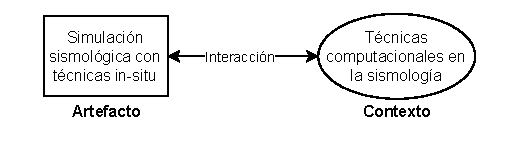
\includegraphics[width=0.9\textwidth]{artifact_context}
  \caption{Tema de investigación}
  \label{fig:artifact}
\end{figure}

\section{Actividades a realizar}
\label{sec:activities}

El marco de trabajo que se utiliza en la ciencia del diseño se presenta en la~\cref{fig:framework}. El contexto social se refiere a aquellas personas que impactan y son impactadas por nuestra investigación. En nuestro caso las personas interesadas son investigadores en sismología, los desarrolladores de bibliotecas in-situ y los desarrolladores de la simulación sismológica SeisSol. El contexto del conocimiento se refiere a las áreas del saber que impactan y son impactadas por el proyecto. En nuestro caso estas incluyen la sismología, las técnicas de análisis y visualización in-situ y la computación de alto rendimiento.

En la ciencia del diseño, un problema de investigación se divide en problemas de diseño y preguntas de conocimiento. Los primeros se resuelven con ciclos de diseño y los segundos con ciclos empíricos. En nuestro proyecto identificamos las siguientes partes:

\begin{itemize}
    \item Pregunta de conocimiento 1 (PC1): ¿Cuáles técnicas in-situ se utilizan en otros dominios de la ciencia a parte de la sismología?
    \item Problema de diseño (PD): La extensión de una simulación sísmica numérica para que utilice el análisis y la visualización in-situ.
    \item Pregunta de conocimiento 2 (PC2): ¿Qué tan efectiva es la herramienta desarrollada en términos de ciencia y rendimiento computacional?
\end{itemize}
Cada una de estas partes corresponde con un objetivo específico del proyecto los cuales reproducimos a continuación:
\begin{enumerate}
  \item Caracterizar simulaciones en otros dominios que hayan incorporado el análisis in-situ. % Explicar que esto terminará en un artículo.
  \item Extender una simulación sísmica numérica para que utilice el análisis y la visualización in-situ. % Explicar que esto incluye el diseño y mejora del rendimiento del programa.
  \item Estudiar el rendimiento y validar la utilidad de la simulación extendida. % Explicar que esto incluirá el criterio de expertos en el área.
\end{enumerate}

El ciclo empírico (CE1) para responder la PC1 tendrá como objetivo el caracterizar simulaciones en otros dominios que hayan incorporado el análisis in-situ. Para realizar esto se llevará a cabo una revisión sistemática de literatura utilizando los parámetros definidos en las recomendaciones PRISMA 2020~\cite{Page2021}. 

% Las actividades relacionadas a este ciclo son las siguientes:
% \newcounter{tasks}
% \begin{enumerate}
%     \item Definir los parámetros de la revisión: Esta actividad incluye la delimitación de la búsqueda, la creación del protocolo de revisión, la selección de bases de datos y las hileras de búsqueda y la definición de los criterios de inclusión y exclusión.
%     \item Llevar a cabo la revisión: Aquí se llevará a cabo la búsqueda de los artículos científicos, así como la aplicación de los criterios de inclusión y exclusión, y la extracción de datos con el protocolo de revisión.
%     \item Análisis de datos: Se analizarán los datos que extrajeron de la revisión y se llegará a conclusiones que se podrán utilizar para informar el desarrollo del proyecto actual.
%     \setcounter{tasks}{\value{enumi}}
% \end{enumerate}
En el ciclo de diseño (CD) para resolver el PD se extenderá la simulación SeisSol para que haga uso de técnicas de análisis y visualización in-situ. Para lograr esto se hará uso del conocimiento obtenido en el CE1 para informar el diseño de la solución, así como el análisis de la base de código y consultas a los autores de la simulación y las bibliotecas de análisis y visualización in-situ. 
Se llevarán a cabo consultas con investigadores del Observatorio vulcanológico y sismológico de Costa Rica (OVSICORI) para definir escenarios de simulación que servirán para validar el funcionamiento de la simulación antes y después de los cambios a realizar, así como su rendimiento computacional. Será necesario entonces ejecutar la simulación sin modificaciones para tener un entendimiento de cómo se comporta esta de manera inicial. Estas pruebas se llevarán a cabo en la supercomputadora Polaris del laboratorio nacional Argonne (ANL) en EEUU. Con esta base, se llevarán a cabo las modificaciones al código, esto se realizará en la sección del programa que realiza el ciclo principal de la simulación utilizando la biblioteca Ascent. Se mantendrá comunicación con la comunidad de desarrolladores de SeisSol para que estén al tanto de estas modificaciones en caso de que se considere que sea provechozo mezclarlas al tronco principal del repositorio. Una vez hechas las modificaciones se llevaran a cabo las pruebas con los escenarios escogido anteriormente, mientras se atienden los problemas que se encuentren gracias a la ejecución de los casos.

Finalmente, en el segundo ciclo empírico (CE2) se responderá la PC2. Se realizarán validaciones de los resultados obtenidos con sismólogos. También se realizarán pruebas de rendimiento computacional, escalamiento fuerte y débil, las cuales servirán para conocer los límites de la herramienta, así como encontrar el overhead de las modificaciones realizadas al código. Las validaciones con los expertos se realizarán mediante entrevistas en donde se evaluará la calidad de la simulación, así como la utilidad percibida de la misma. En cuanto a las pruebas de rendimiento computacional, se 

De forma transversal se estará documentando el avance del proyecto.

\begin{figure}[h]
    \centering
    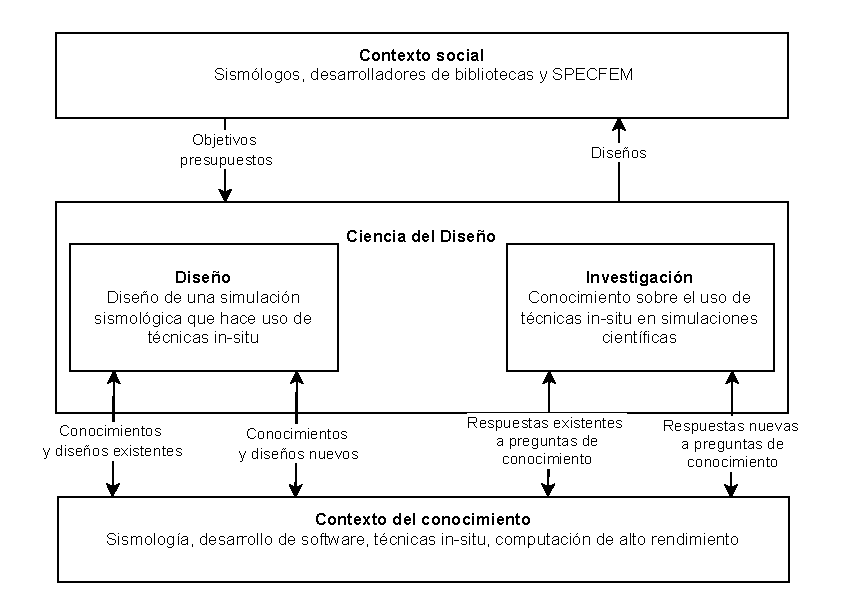
\includegraphics{framework}
    \caption{Marco de trabajo en el que se desarrolla la investigación}
    \label{fig:framework}
\end{figure}

\section{Cronograma}
Las actividades definidas en el~\cref{sec:activities} se llevarán a cabo según el cronograma que se encuentra en la~\cref{fig:chronogram}.

\begin{figure}
    \centering
    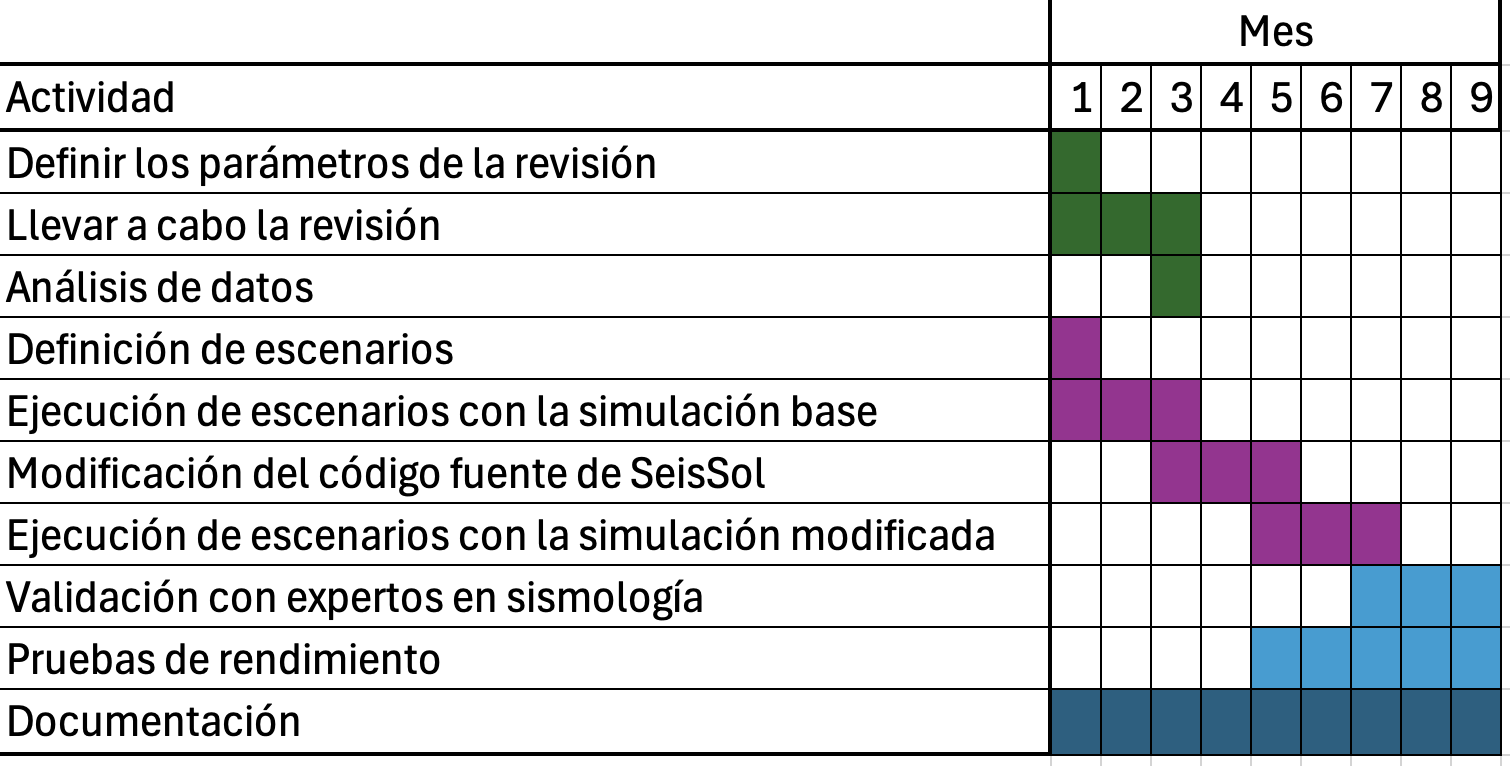
\includegraphics[width=0.7\textwidth]{chronogram}
    \caption{Cronograma tentativo para el desarrollo del proyecto.}
    \label{fig:chronogram}
\end{figure}

\printbibliography

\end{document}
